\documentclass{article}
\usepackage{ctex}
\usepackage{float}
\usepackage{geometry}
\usepackage{amsmath}
\usepackage{graphicx}
\geometry{a4paper, scale=0.8}

\title{ISOA Midway Report}
\author{Group "200"\\YiDai 2017013562\\ZhaohengLi 2017050025}

\begin{document}
\maketitle

\section{项目介绍}
我们以疫情部分的舆论方面为核心,提取舆论主题,结合时间线展示群众的关注点变化,对访问者提供舆论谣言判断服务。同时我们也注意到,信息服务平台如果缺失一方面的关键信息很容易丧失吸引力,我们还会实现政府的相关措施发布、并实现确诊数据展示。

主要实现目标如下:
\begin{itemize}
	\item{\textbf{疫情展示}} 主要包括疫情确诊地图、详细数字和相关新闻或政策的时间线。
	\item{\textbf{舆情关注展示}} 对舆情进行主题提取,结合时间线展示群众的关注点变化
	\item{\textbf{虚假新闻/谣言判断及搜索}} 用户输入文本,对文本进行分析,为用户提供相关已证实谣言或者相关新闻,并给出用户输入文本为谣言的概率。
\end{itemize}

\begin{figure}[H]
\centering
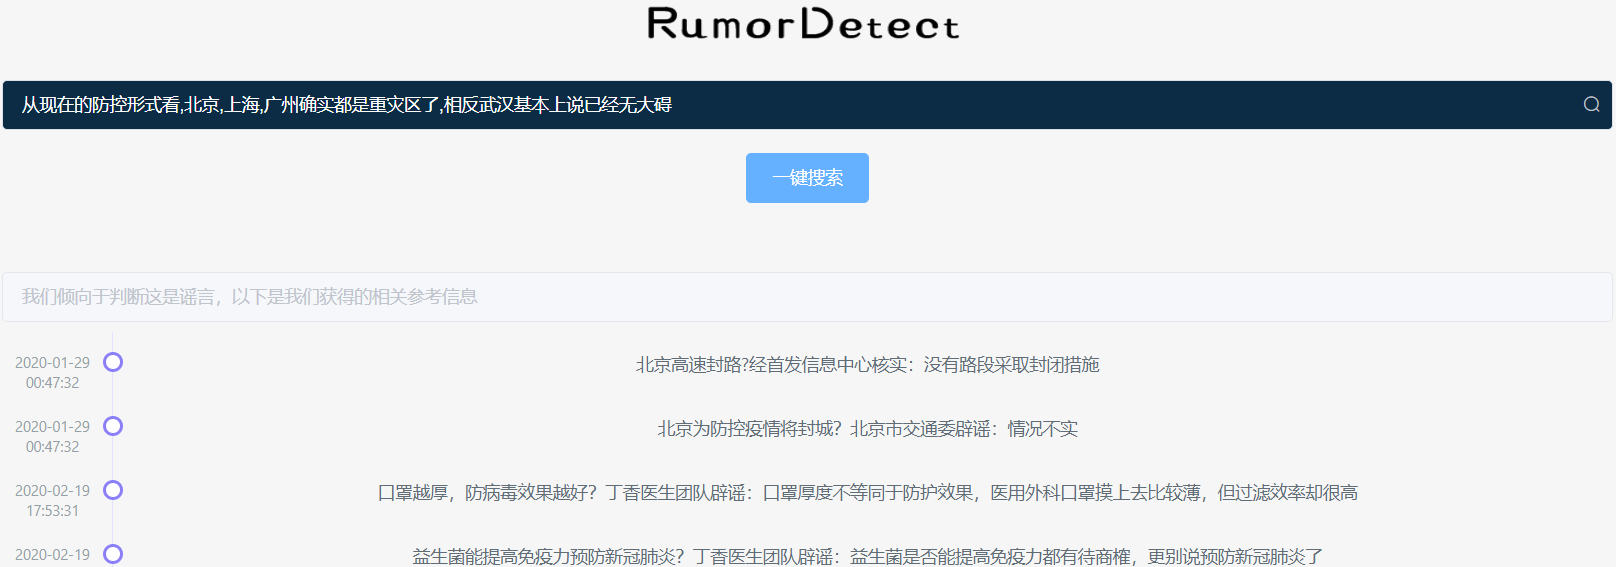
\includegraphics[width=0.8\textwidth]{pic0.png}
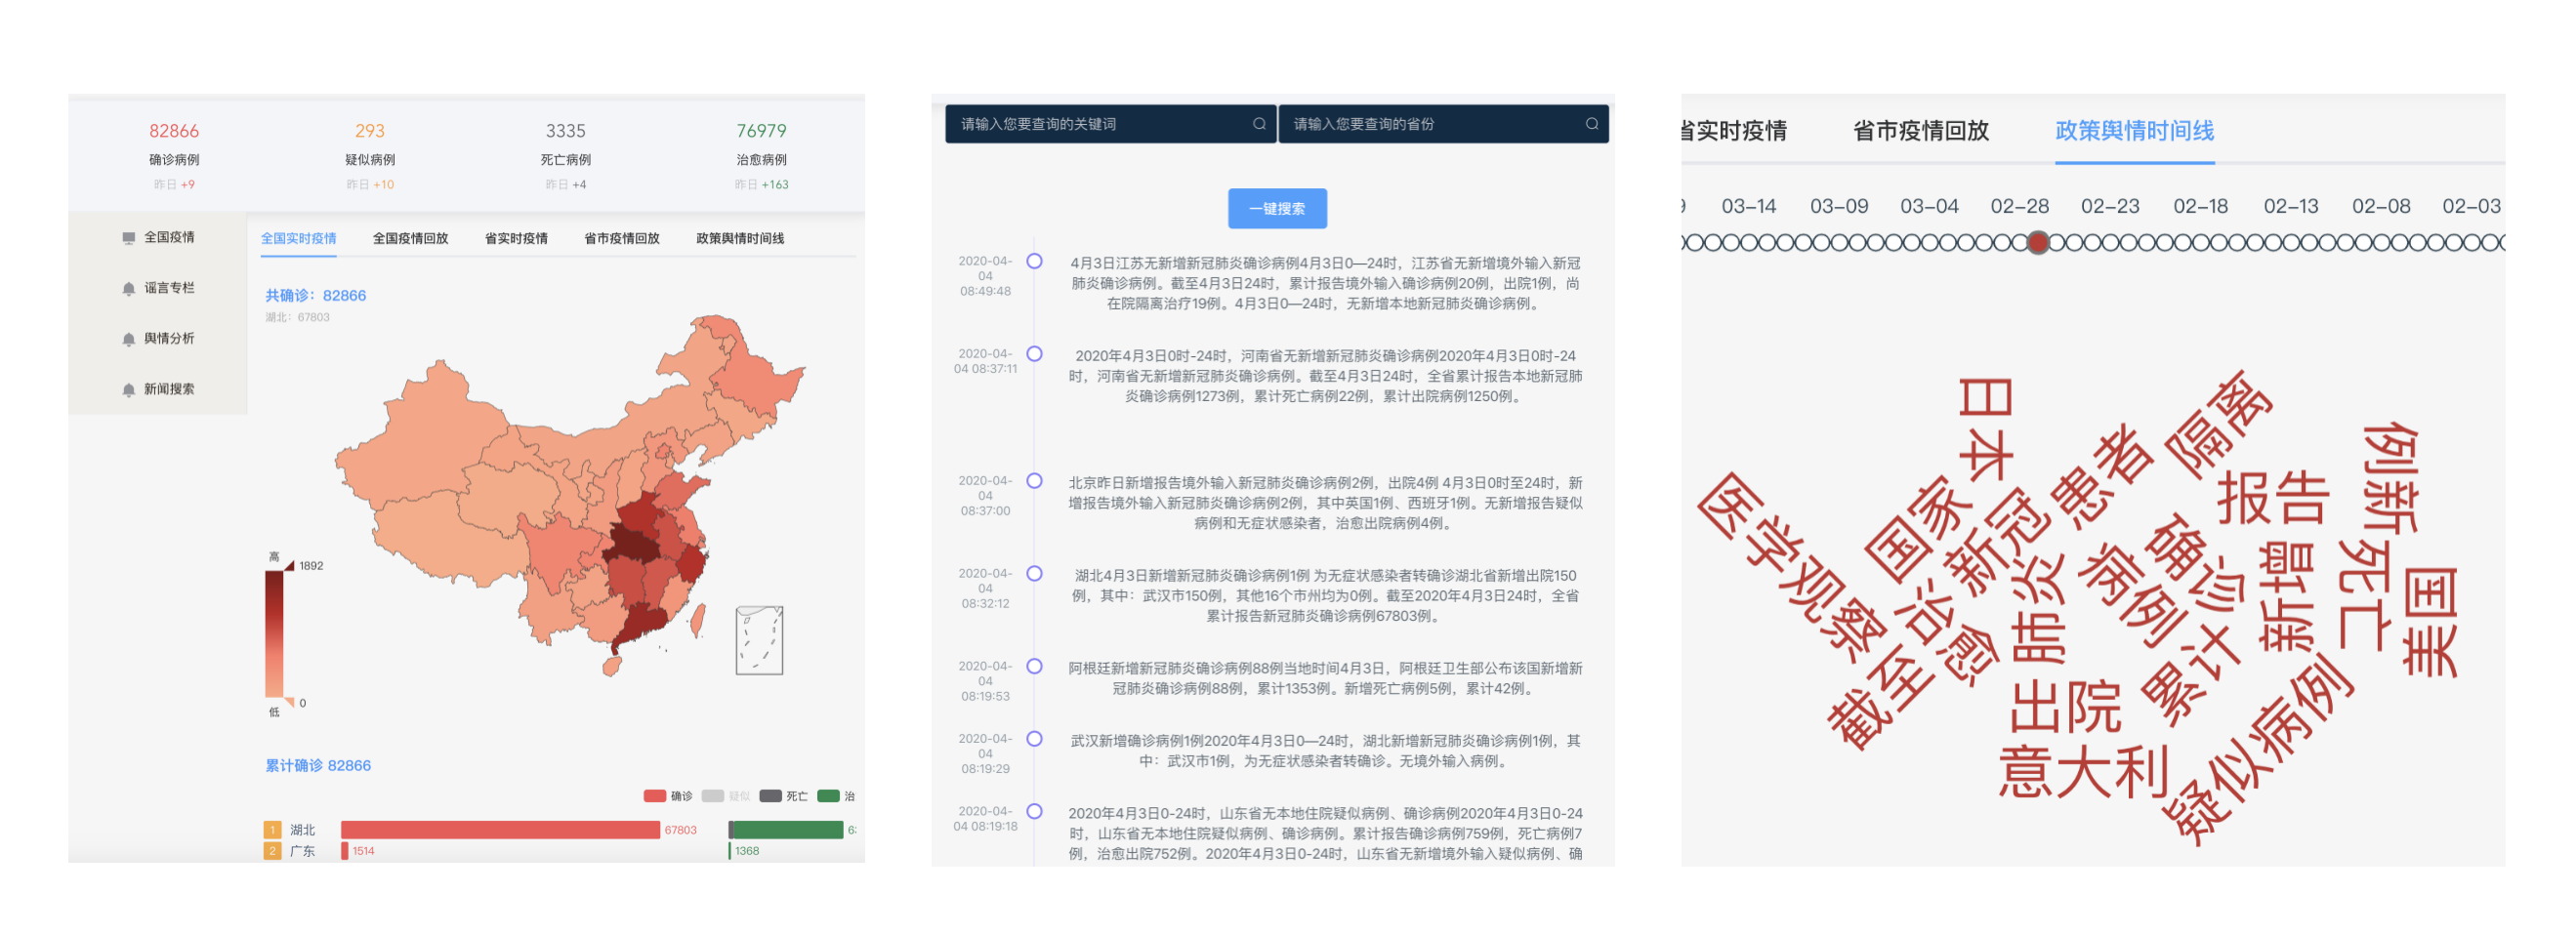
\includegraphics[width=0.9\textwidth]{pic1.png}
\end{figure}

\section{项目特点}
\begin{itemize}
	\item{\textbf{疫情时序数据的维护与展示}\\
	目前主流信息平台微博客户端、新闻网站等提供的信息主要为即时疫情信息,当用户需要了解疫情舆论发展动态或梳理疫情发展趋势时,这就需要使用长时间记录的时序数据,并且目前这种长期的变化数据并不容易获取。}
	\item{\textbf{互动性的舆论判别以及结合人工智能判别与相关真相/谣言推荐的谣言判断系统}\\
	支付宝等平台给出了一些新闻真伪的数据,但它的吸引力并不如它的可靠度那么高。我们更希望获取实时、实地有关的舆论判别,并通过互动式的舆论判别来知道一些自己关心事项的真实程度,并结合政策动态来作出决策。}
	\item{\textbf{在舆论发展序列中提取群众关注热点变化}}\\
	通过对各大平台上发布的新闻、评论数据进行收集,分析群众关注热点在时序上的变化,展示舆论热点随时间上的迁移。



\end{itemize}

\section{用户群体}
\begin{itemize}
	\item{希望获得“热搜”以外长期信息的用户。}
	\item{获取信息来源较少、受“浙江十万只鸭派往巴基斯坦治蝗”、“双黄连口服液可抑制新型冠状病毒”等即时热搜影响较大的用户。}
	\item{对地区(不仅限当地)信息、政策更关心的用户。}
	\item{希望利用疫情发展、群众舆论与关注点发展变化的用户。}
\end{itemize}

\section{项目结构}
\begin{figure}[H]
\centering
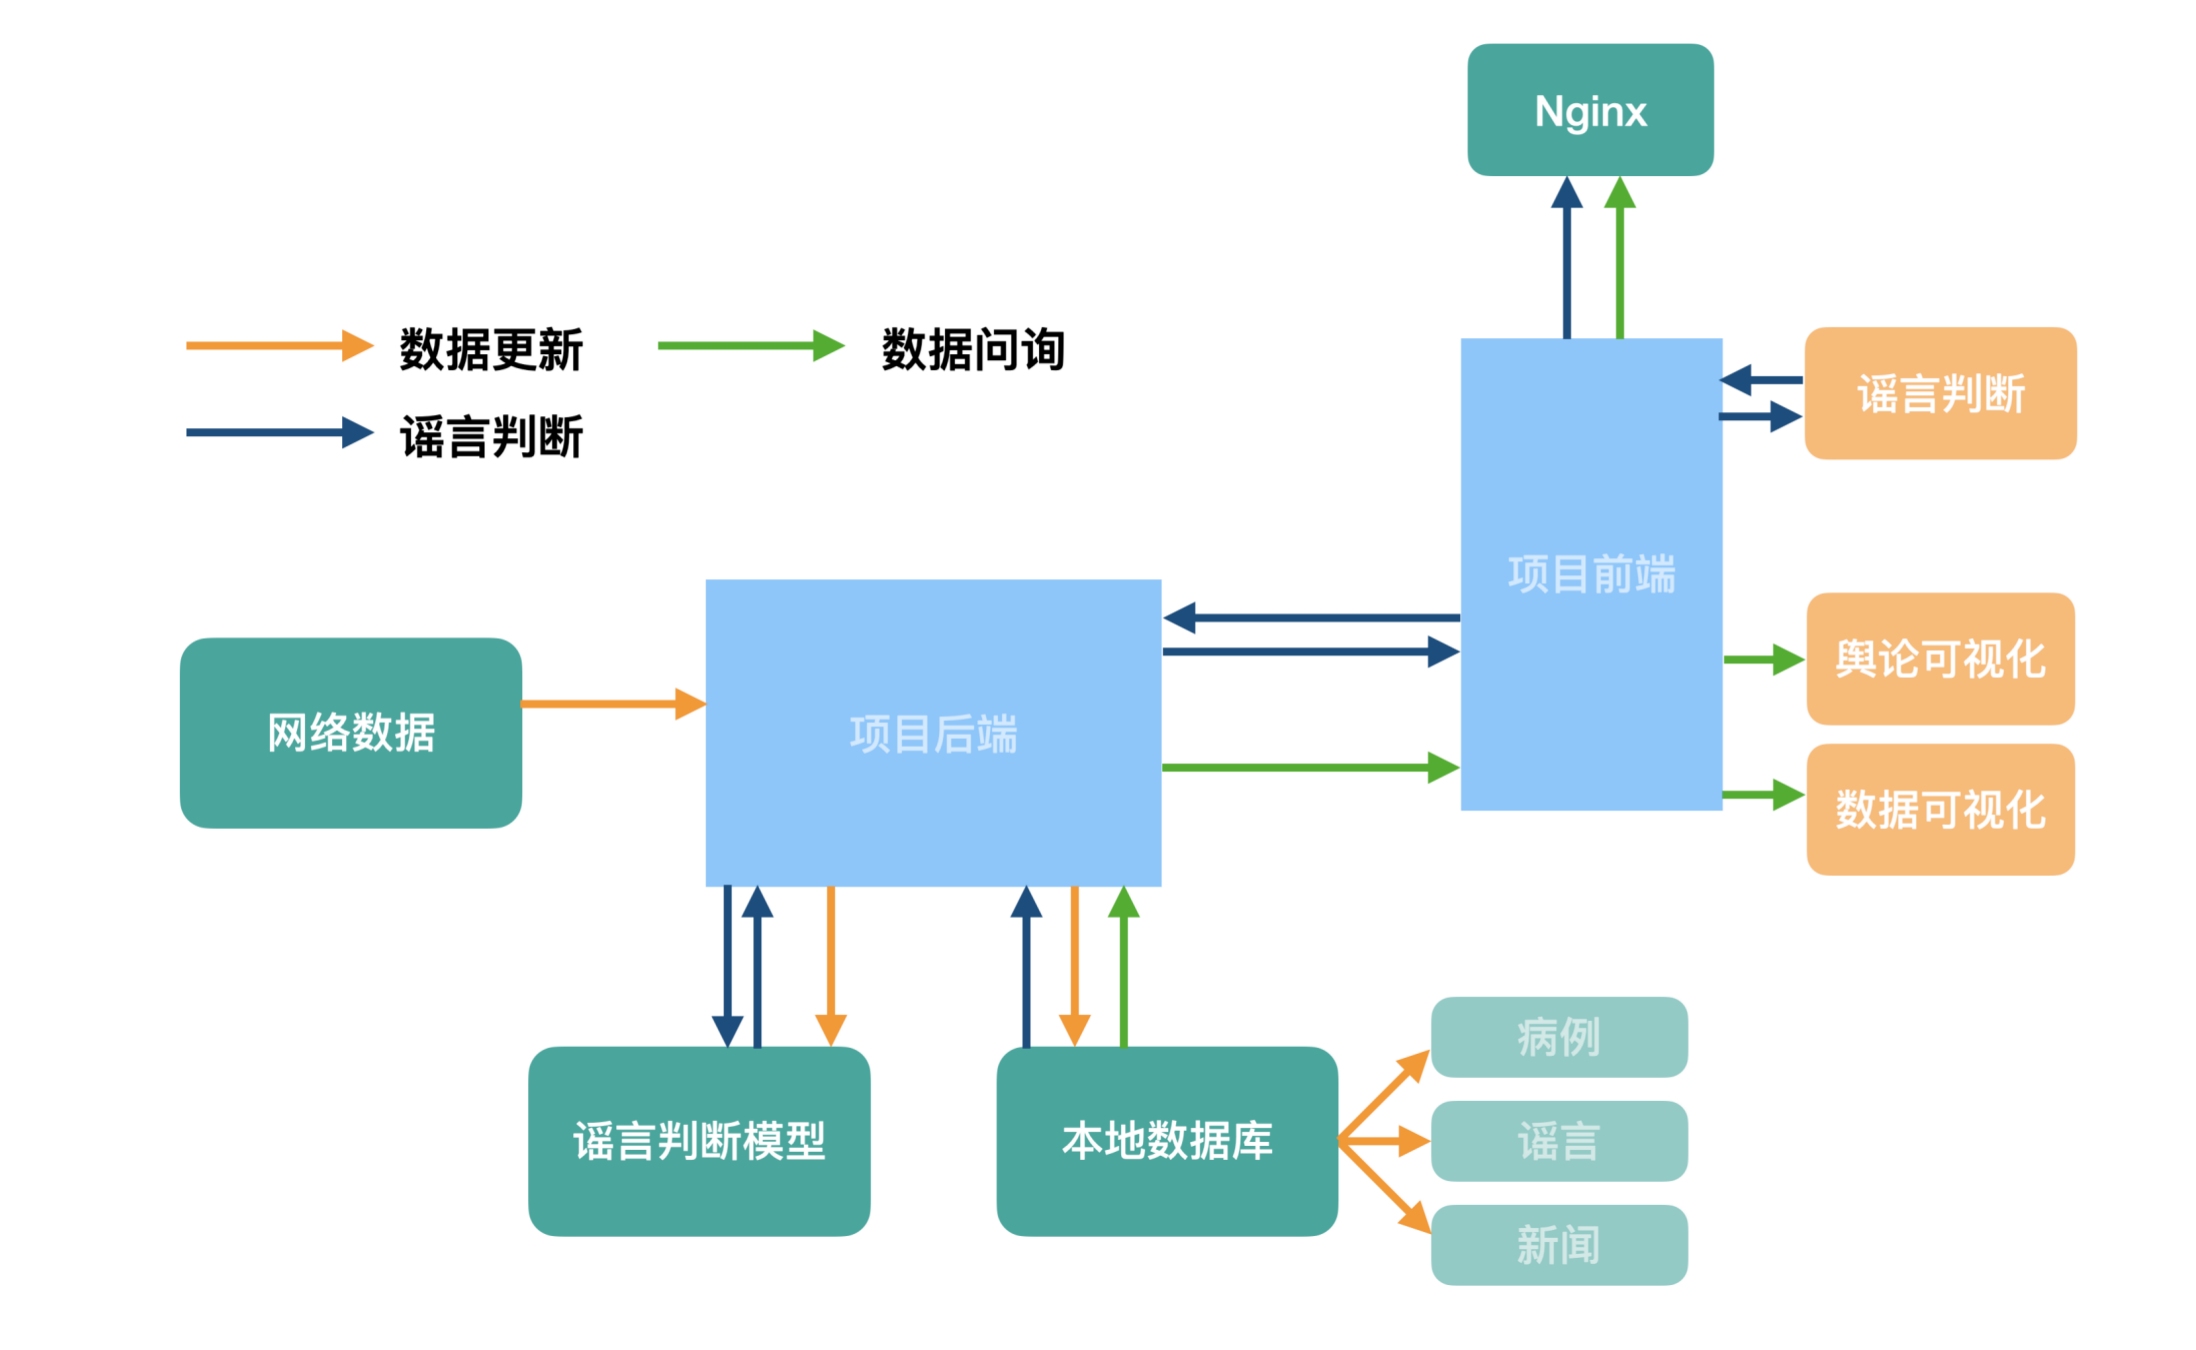
\includegraphics[width=0.8\textwidth]{pic2.png}
\end{figure}

\section{关键技术}
\subsection{谣言判断}
\begin{itemize}
	\item{词粒度语义信息提取}
	\item{多头注意力+卷积轻量级模型挂载服务}
	\item{相关谣言辅助识别}
\end{itemize}

\subsection{舆论热点迁移}

\begin{itemize}
	\item{LDA主题模型提取舆论中的关注热点}
	\item{对指定时间粒度上的舆论进行综合分析以及话题提取}
	\item{对话题的“生命周期”、“生长趋势”以及“活跃程度”进行分析}
	\item{对各个热点或话题的交替浮现进行分析与展示}
\end{itemize}


\section{项目计划}
\begin{figure}[H]
\centering
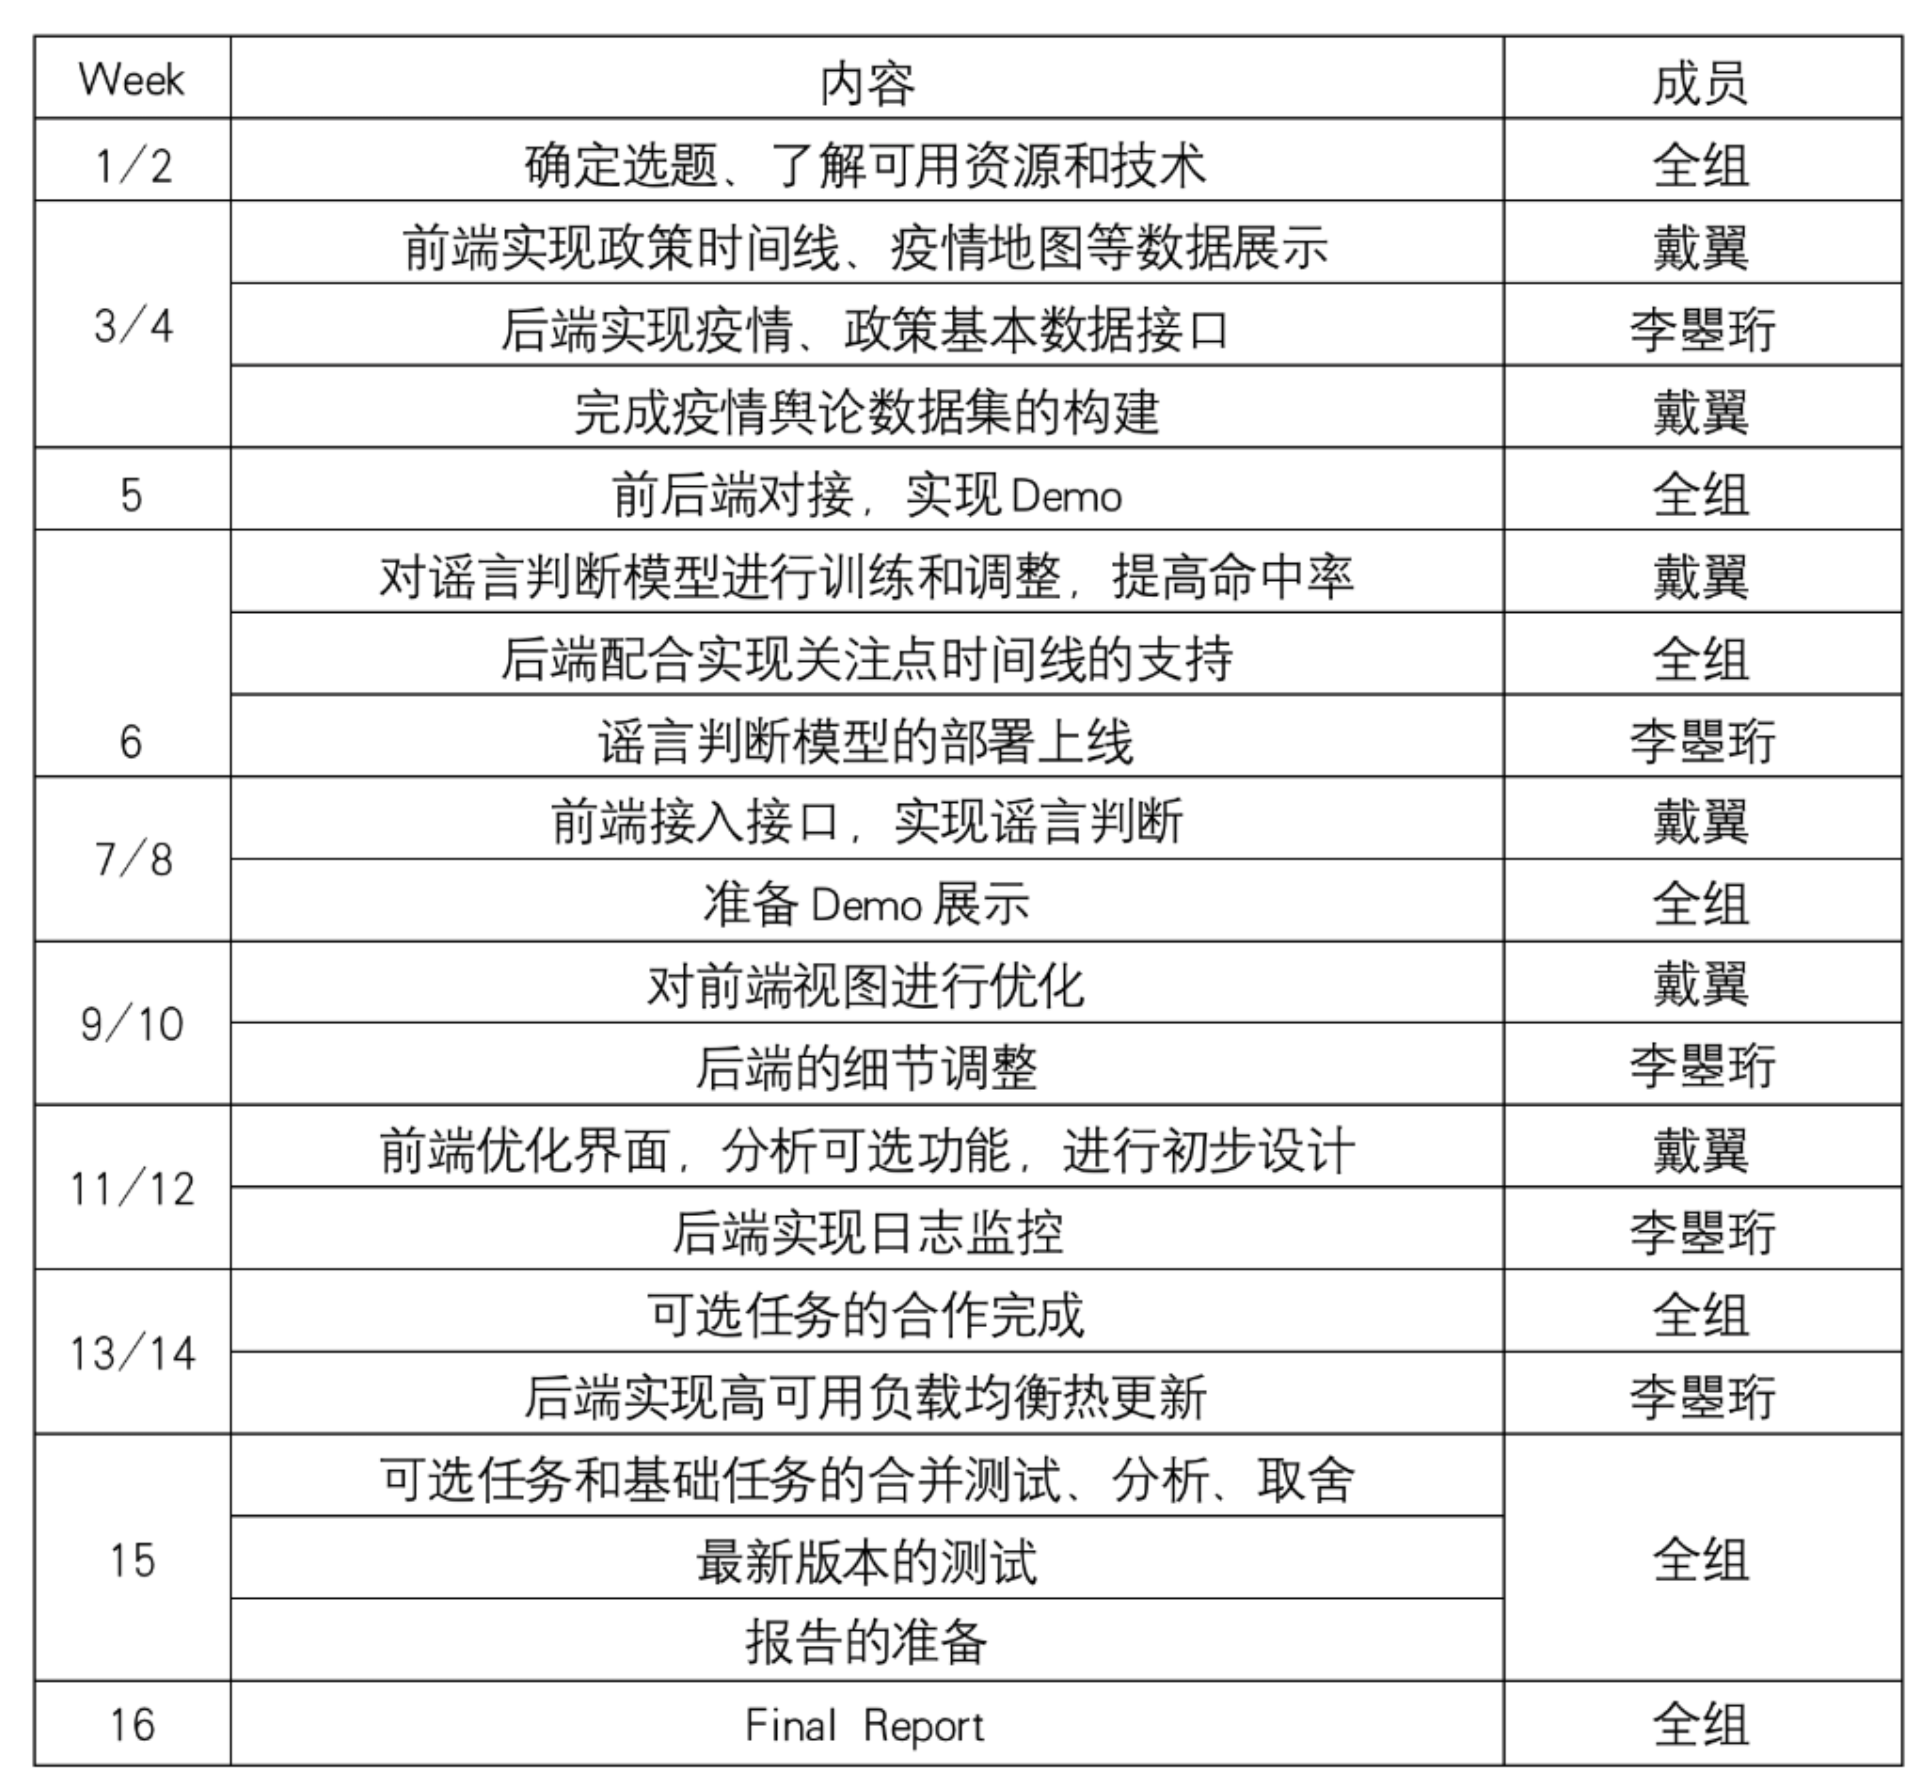
\includegraphics[width=0.8\textwidth]{pic3.png}
\end{figure}

\section{项目进展}
\subsection{前阶段工作总结}
目前为止,我们按照初期制定的工作计划稳步前进,已经将目标功能全部实现,即疫情确诊地图信息、详细数据和相关新闻或政策的时间线展示,对舆情进行主题提取以及结合时间线展示群众的关注点变化分析及展示,最后,完成对用户输入文本进行分析,为用户提供相关已证实谣言或者相关新闻,并给出用户输入文本为谣言的概率。

在这过程中遇到的问题主要有以下两个。

在舆论热点迁移的分析过程,由于我们获取的新闻数据内容比较单一,导致每个时间粒度下提取出的热点、话题内容比较相似,迁移程度不太明显。对此的解决办法是多方大量再收集数据,我们将会从微博上爬取相关的新闻、用户的评论等信息来丰富我们的数据库。

在域名申请的过程中,我们被告知个人性质的网站是不能展示疫情数据的,因此我们的备案不能通过。这个问题我们将会在后续过程中同助教协商,寻找解决办法。


前阶段工作的分工以及合作情况在项目计划表中有详细注解,未来工作的分工也会按照计划表有序进行。


\subsection{前阶段工作评价与分析}

总体来看,我们如期地完成了工作计划,主要功能全部实现,网站内容丰富、功能完整、版面设计合 理,能够给用户较为良好的体验。 

但是通过小组互评我们也发现了自己的缺点。通过展示Q\&A和事后Peer Review,我们分析与统计了获得的评估,发现了目前的缺点。我们面对的意见大致有四类(见下图)。

\begin{figure}[H]
\centering
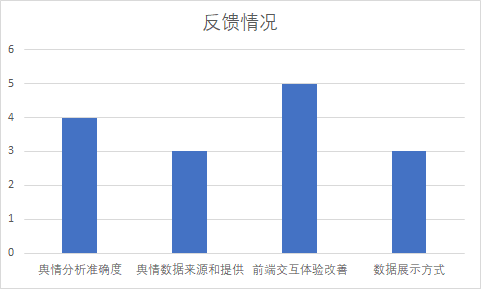
\includegraphics[width=0.8\textwidth]{pic4.jpg}
\end{figure}

一是舆情分析准确度,谣言模型产生的结果未必可信,除了展示相关谣言,我们也许需要一个更合理的方式把分析结果呈现出来,我们会在下一阶段工作中去修正这个问题。

二是舆情数据来源(包括筛选算法)和提供,舆论数据内容单一也是我们的缺点,在下一阶段的工作中,我们将会从微博上爬取相关的新闻、用户的评论等信息来丰富我们的数据库,也会进一步完善原有的筛选算法。

三是前端交互体验改善建议,我们获得了”内测用户“宝贵的意见,这是来自用户角度的观点,例如用”Loading“来填充等待时间的空白屏。这些建议,我们已经开始权衡利弊进行修改。下一次milestone是在12周,而我们原本计划在9/10周展开前端优化,我们可以按照计划优化,事后进行第二次用户调研。

四是数据展示方式的问题,有的意见中希望有更多的数据形式。我们在报告过程中分析了前面主要做舆论分析的一组(JustDropIt),他们的词云和弹幕都很具有观赏性、也有很好的热度分析曲线,我们会考虑借鉴一二,这需要前端添加Feature和后端增加数据接口,已经加入了我们9/10周的工作清单。

意见中也有一些问题其实我们已经解决,例如”实时疫情的最后更新时间“,不过我们也在思考是不是在前端版面中不够显眼,使得用户存在疑问,这个问题也已经放入我们第11周获取用户调研的工作清单。

\subsection{未来工作计划}
目前项目按照初期制定的工作计划稳步前进,接下来的计划不会有大的改变,但会增加以下内容:
\begin{itemize}
	\item{多方获取数据丰富舆论数据集}
	\item{改善前端呈现方式与交互体验 提供亮点 找出重点}
	\item{优化舆论热点迁移的分析过程以及展示方式}
	\item{进行用户实验并听取用户感受再次改进项目}
\end{itemize}


\end{document}